\subsection{User Interfaces}

\subsubsection{Windows Client}
The user interface was developed to have a native Windows look and feel from the beginning of the project. 
This means that anything superfluous has been removed, and that the content of the \texttt{DriveIT Windows Client} is in focus. 
The \texttt{Employee} needs to finish his/her task as quickly and efficiently as possible, which extra unnecessary user interface elements would hinder.
Motion has also been introduced in the interface in the form of user interface transitions when navigating menus. 
This all follows the Design Guidelines of Microsoft\footnote{\url{http://msdn.microsoft.com/library/windows/apps/hh781237.aspx}}.

The interface could have been more refined and made easier to use. The input fields for creating and updating entities could have fetched and parsed data dynamically, depending on the user context. 

When creating a \texttt{Sale} the "Car Id" field could present more meaningful selection options for the \texttt{Employee} e.g. model names with an attached ID. Currently the user has to know the ID in advance. \\
This goes for all entities.

\subsubsection{Prototyping}
A prototype was sketched and refined over the course of the project.\\
The final prototype can be seen below.\\

\textbf{Main Window:}
\begin{figure}[H]
	\centering
	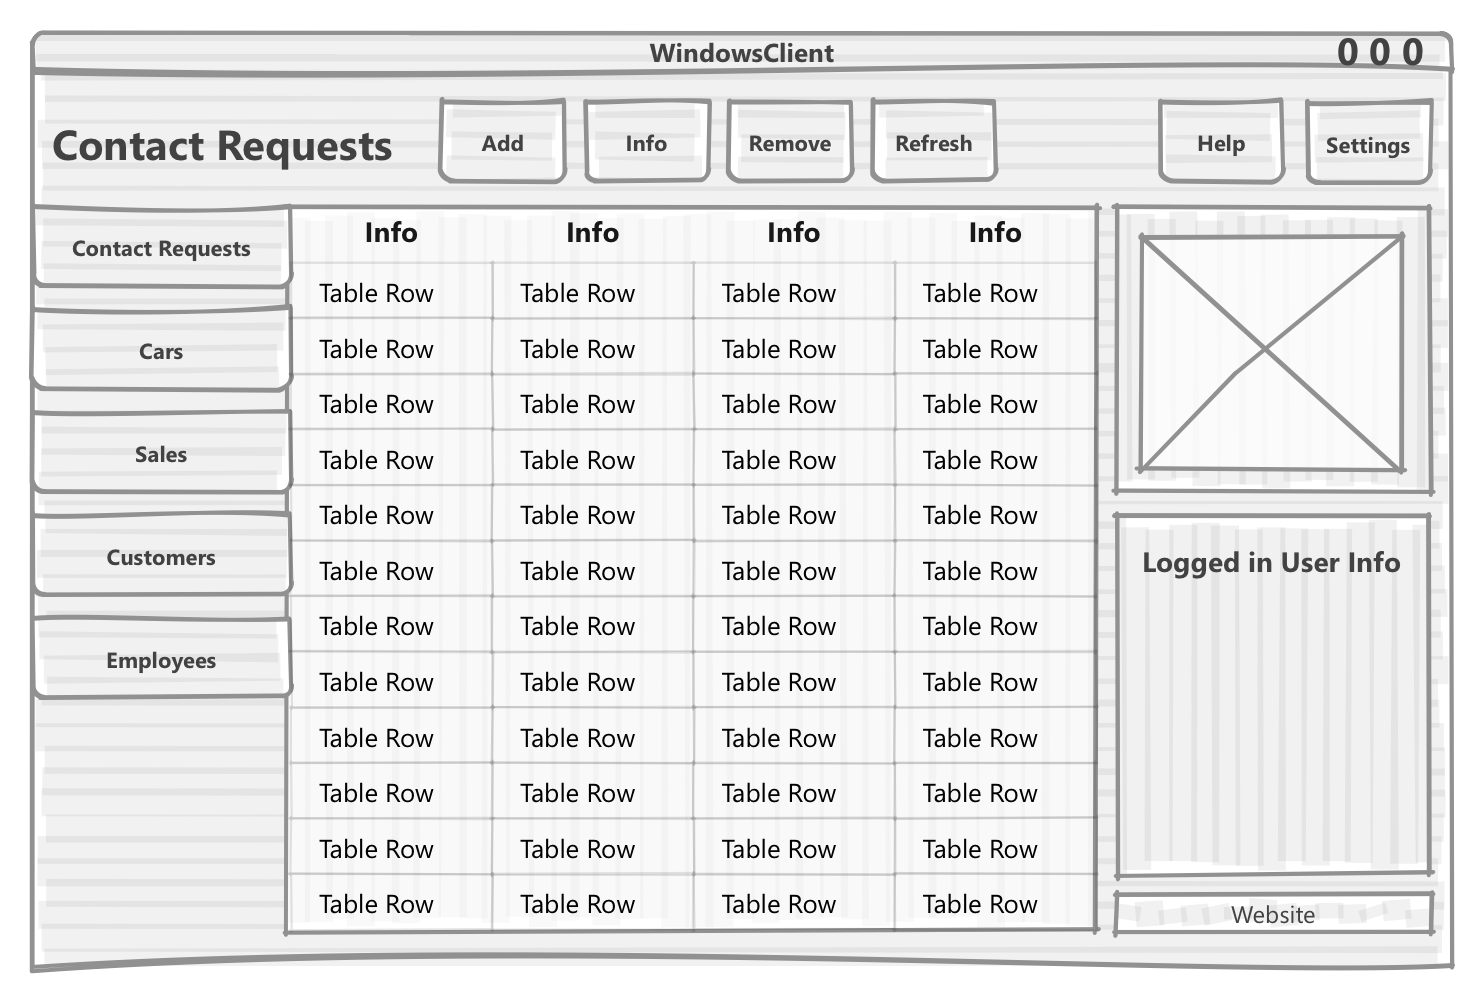
\includegraphics[scale=0.25]{Figures/UserInterface/WindowsMain}
	\caption{The Sketch of the Main Window of the Windows Client.}
	\label{fig:UserInterfaceWindowsMain}
\end{figure}
\textbf{Entity Windows:}
\begin{figure}[H]
	\centering
	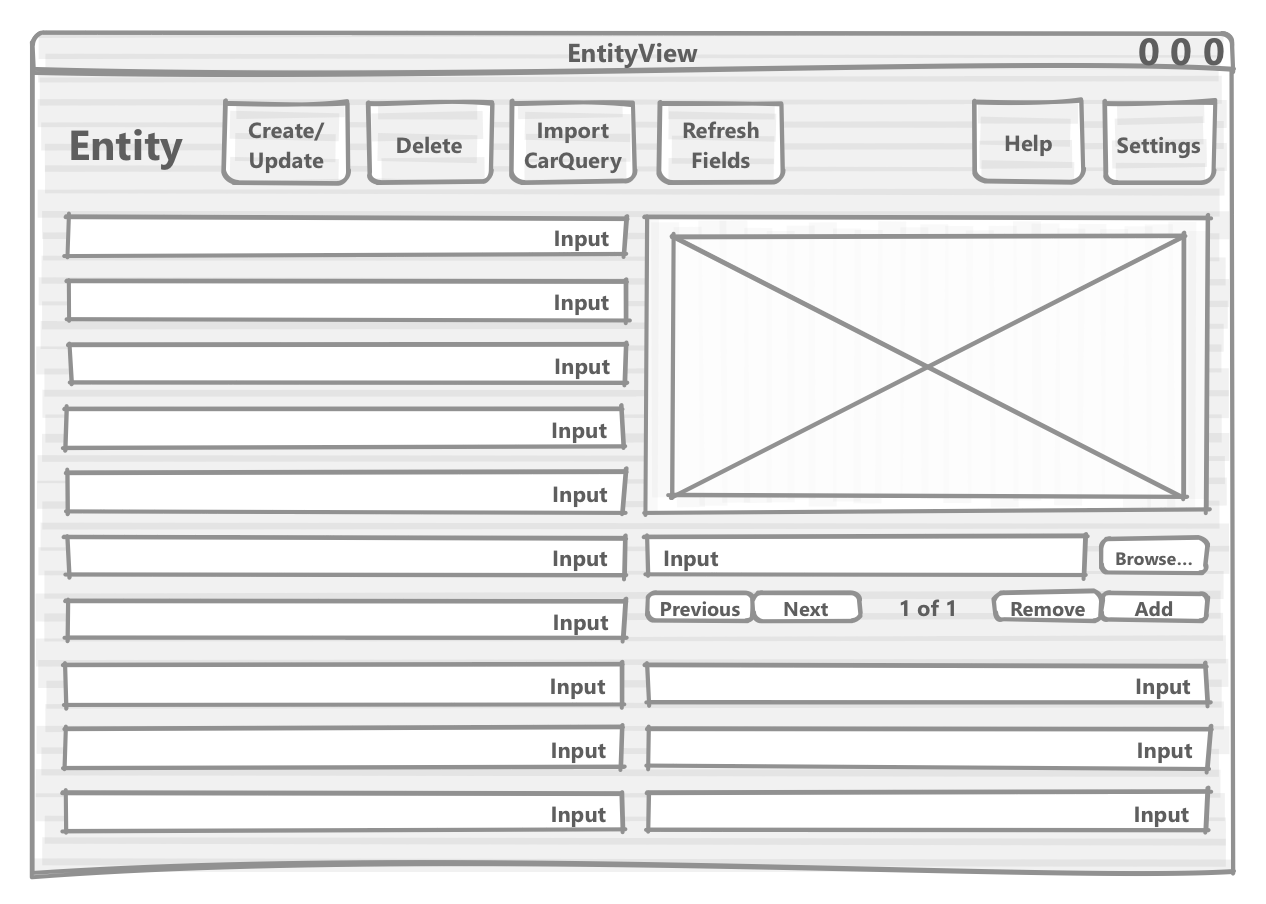
\includegraphics[scale=0.30]{Figures/UserInterface/EntityView}
	\caption{The Sketch of the Entity View of the Windows Client.}
	\label{fig:UserInterfaceEntityWindow}
\end{figure}
